\documentclass[final,hyperref={pdfpagelabels=false}]{beamer}
\usepackage{grffile}
\mode<presentation>
  {
  %  \usetheme{Berlin}
  \usetheme{I6pd2}
  }
  \usepackage{times}
  \usepackage{amsmath,amsthm, amssymb, latexsym, multicol}
  \boldmath
  \usepackage[english]{babel}
  \usepackage[latin1]{inputenc}
  \usepackage[orientation=portrait,size=custom,width=60,height=90,scale=1.4]{beamerposter}  
  
  % my packages
  
  %%%%%%%%%%%%%%%%%%%%%%%%%%%%%%%%%%%%%%%%%%%%%%%%%%%%%%%%%%%%%%%%%%%%%%%%%%%%%%%%%5
  %\graphicspath{{figures/}}
  \title{SyVOLT: Full Model Transformation Verification Using Contracts}
  
  \author{Levi L\'{u}cio, Bentley James Oakes$^{\dagger}$, Cl\'{a}udio Gomes$^{\ddagger}$, Gehan Selim$^{\star}$,
  Juergen Dingel$^{\star}$,
  James R. Cordy$^{\star}$, and
  Hans Vangheluwe$^{\dagger\ddagger}$
  }
  
  \institute[McGill, Antwerp, Queen's]{$^{\dagger}$McGill University, Montreal, Canada\qquad
       $^{\ddagger}$University of Antwerp, Belgium
       $^{\star}$Queen's University, Kingston, Canada}
  
  \date{\today}


  %%%%%%%%%%%%%%%%%%%%%%%%%%%%%%%%%%%%%%%%%%%%%%%%%%%%%%%%%%%%%%%%%%%%%%%%%%%%%%%%%5
  \begin{document}
  \begin{frame}{}
      \vspace{-2.7cm}
        \begin{block}{\normalsize Abstract}
        \footnotesize
   		We introduce SyVOLT, a plugin for the Eclipse
   		development environment for the verification of structural pre-/post-condition contracts on model transformations. The plugin
   		allows the user to build transformations in our transformation
   		language DSLTrans using a visual editor. The pre-/post-condition
   		contracts to be proved on the transformation can also be built in
   		a similar interface. Our contract proving process is exhaustive,
   		meaning that if a contract is said to hold, then the contract will
   		hold for all input models of a transformation. If the contract does
   		not hold, then the counter-examples (i.e., input models) where the
   		contract fails will be presented.
   		Demo: \url{https://www.youtube.com/watch?v=8PrR5RhPptY}
        \end{block}
        
\vspace{-0.2cm}
    \begin{block}{SyVOLT Highlights}
    

    \vspace{-2.2cm}
            \begin{columns}[t,totalwidth=\linewidth]
             \begin{column}{.19\linewidth}
             \footnotesize
           \begin{center}\textbf{Input Independence and Exhaustiveness}\end{center}
           \footnotesize
           If a pre-/post-condition contract holds for a model transformation, a formal guarantee
           exists that whenever a transformation's input model contains
           the pattern in the pre-condition of the contract,
           the output model will contain the pattern
           in the contract's post-condition~\cite{Lucio2014}. Contracts can optionally include traceability relations between input and output
           patterns. \\~\\
           
           \end{column}
           \hspace{-1.2cm}\vrule\hspace{.05cm}
           \begin{column}{.175\linewidth}
           \footnotesize
          \begin{center}\textbf{Push-Button Proofs}\end{center}
          \footnotesize
            Fully automatic and the approach's formal details are completely hidden from the user. Property proving process will automatically
            create all required artifacts, run
            the process, and provide the results to the user within the
            Eclipse environment. User always stays within the Eclipse
            environment when developing the contracts and the model
            transformations.
            \end{column}
            \hspace{-1.2cm}\vrule\hspace{.05cm}
            \begin{column}{.16\linewidth}
                        \footnotesize
                      \begin{center}\textbf{Proving Contracts about ATL Model Transformations}\end{center}
                      \footnotesize
                       
                        To prove contracts on ATL transformations,
                        we have built a higher-order transformation that
                        automatically transforms declarative ATL transformations
                        into semantically equivalent DSLTrans~\cite{Oakes} ones. In the
                        future we will couple this higher-order transformation with
                        SyVOLT's user interface.
                        \end{column}
            \hspace{-1.2cm}\vrule\hspace{.05cm}
            
            
            
            
            \begin{column}{.19\linewidth}
         \footnotesize
                   \begin{center}\textbf{Scalability and Speed}\end{center}
                   \footnotesize
            We have verified contracts on DSLTrans transformations with over 60
            rules, and ATL transformations with up to 13 rules~\cite{Oakes}. A DSLTrans transformation
            is composed of 10 up to about 50 rules, while an
            ATL transformation is around 20 rules~\cite{wimmer13}. Even though
            our technique is exhaustive, verification can be performed within seconds. Further works: ~\cite{Selim2015, Selim2014}.
            \end{column}
            \hspace{-1.2cm}\vrule\hspace{.05cm}
            \begin{column}{.18\linewidth}
                        \footnotesize
                      \begin{center}\textbf{Based on Symbolic Execution}\end{center}
                      \footnotesize
                        Each symbolic execution - a path condition - is a
                        finite representation of the execution of a subset of the transformation's
                        rules on the infinite set of input models. 
                        Contracts of interest are proved on the set of path conditions
                        and are extrapolated to the
                        infinite set of the model transformation's computations through
                        an abstraction relation~\cite{Lucio2014}.
                        \end{column}
                        
                  \end{columns}
                  
                  \vspace{-0.9cm}
            \end{block}
	\vspace{-0.2cm}
        \begin{block}{Integration with Eclipse / Graphical Modelling}
        \vspace{-2cm}
        \begin{columns}[t,totalwidth=\linewidth]
         \begin{column}{.585\linewidth}
         \vspace{-1.4cm}
         \small
       \begin{center}\textbf{~}\end{center}
       \footnotesize
%       To take advantage of the Eclipse ecosystem, SyVOLT
%       integrates with the Eclipse Modeling Framework to represent models in a multitude
%       of syntaxes, from graphical to textual. Modellers may then
%       operate in their preferred syntax.
                  
        \begin{center}\textbf{Counter-Examples}\end{center}
        
      When a contract does not hold on a model
      transformation, SyVOLT can pinpoint where the contract's violation occurs by showing the set of model transformation rules used to build a particular path condition for which
      the contract fails. A counter-example is any input model where
      this set of rules would execute. For example, the sample output
      below alerts the user that the contract \textit{motherFather} will
      fail when only the \textit{mother} and \textit{father} rules execute in the
      transformation.\newline
      \footnotesize
      \texttt{
$>$ Contract ``daughterMother'' holds for all input models!\\
$>$ Contract ``motherFather'' does NOT hold for all input
models! The contract fails on the following Path Conditions:\\
$\lbrack$'RootRule\_FatherRule\_MotherRule', \dots$\rbrack$\\
$>$ The smallest Path Conditions where the contract fails are:\\
$\lbrack$'FatherRule\_MotherRule'$\rbrack$\\
$>$ Time to verify 2 contracts: 11.6834638966 seconds.
     }
                  
       \end{column}
       \begin{column}{.385\linewidth}
       %\vspace{5cm}
       %\small
      \begin{center}
      \footnotesize
      \textbf{Eclipse Frontend}
      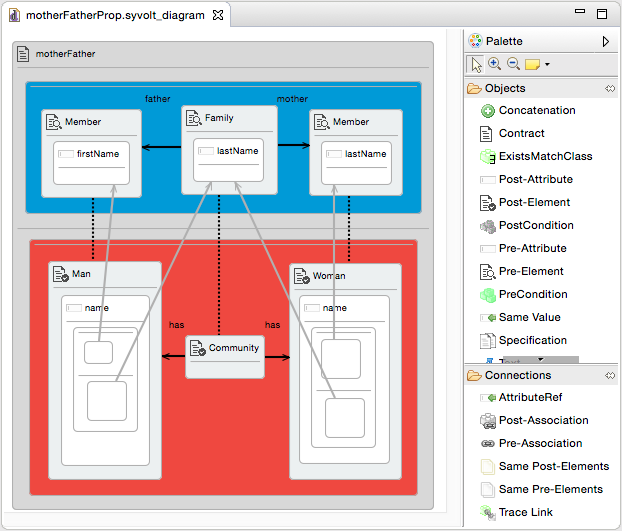
\includegraphics[height=15cm]{figures/eclipse_frontend}
      \end{center}
        %\footnotesize
        
       
        \end{column}
              \end{columns}
        \end{block}
      
      \vspace{-1.7cm}
    \begin{columns}[t,totalwidth=\linewidth]
    \centering
      \begin{column}{1\linewidth}
        \begin{block}{Architecture}
         \vspace{-.8cm}
        \small
        %\begin{center}\textbf{Constant Folding}\end{center}
        \begin{columns}[c,totalwidth=\linewidth]
        \begin{column}{.40\linewidth}
        \begin{center}
        \vspace{-2cm}
        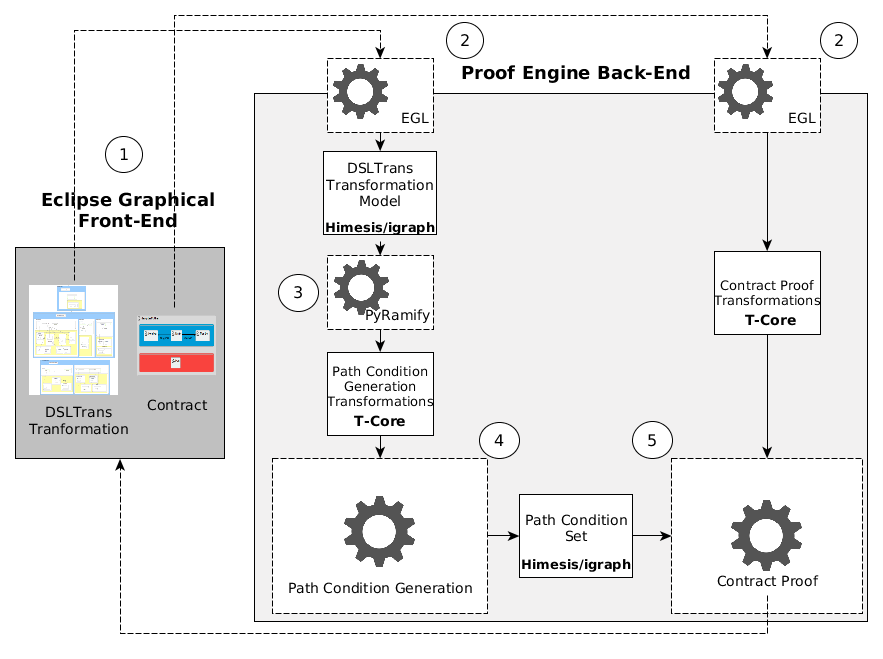
\includegraphics[height=13.4cm]{figures/tooling_arch}\\
        %\footnotesize \textit{Model before}
        \end{center}
        \end{column}
        \begin{column}{.585\linewidth}
        \begin{center}
        %\vspace{-2cm}
%        \includegraphics[width=0.7\linewidth]{images/models/Const1_export}\\
%Model-driven development tools used in SyVOLT's development:

\begin{enumerate}
\setlength\itemsep{1pt}
\setlength{\parskip}{0pt}
\footnotesize
\item SyVOLT Contract Editor - Eclipse Graphical Modeling Framework plugin
\begin{itemize}
\footnotesize
\item Allows for building of DSLTrans transformations and contracts.
\end{itemize}
\vspace{-10pt}
\item Generating Rule and Contract Artifacts
\begin{itemize}
\footnotesize
\item Epsilon Generation Language is used to convert Ecore
models of rules and contracts into igraph-based models to be processed by Python scripts
\end{itemize}
\vspace{-10pt}
\item Generating Artifacts for Path Condition Construction
\begin{itemize}
\footnotesize
\item T-Core model transformation primitives created by EGL for path condition generation
\end{itemize}
\vspace{-10pt}
\item Path Condition Generation
\begin{itemize}
\footnotesize
\item All valid combinations of rules are generated by the Python script
\end{itemize}
\vspace{-10pt}
\item Contract Proof
\begin{itemize}
\footnotesize
\item Contracts are matched onto produced path conditions and output is presented to user
\end{itemize}

\end{enumerate} 

\vspace{2.6cm}
        %\footnotesize \textit{Model after}
        \end{center}
        \end{column}
        \end{columns}
       
       \vspace{-3cm}
        \end{block}
        
      \end{column}
\vspace{0.1cm}
    

    \end{columns}
%    \begin{columns}
%     \begin{column}{0.99\linewidth}
                
%                 \vspace{-0.2cm}
%                 \begin{block}{Conclusions \& Future Work}
%                 \footnotesize
%            	   The optimizations shown here demonstrate how the performance of a model simulation can be increased (as for the constant folding optimization), and how the visual layout of a model can be improved (as with the dead-block removal and flattening optimizations). Our framework allows these optimizations to be specified and implemented easily, and for model optimization to be on the order of seconds.
%            	   
%            	   \footnotesize
%            	   \textbf{Acknowledgments}\\
%            	   We would like to thank Joachim Denil (NECSIS), Bart Pussig (University of Antwerp), and Pieter Mosterman (The Mathworks) for their support.
%                 \end{block}
                 \vspace{-0.2cm}
                 \begin{block}{Bibliography}
%                 \footnotesize
%         	   \begin{thebibliography}{10} 
         	   \vspace{-2.1cm}
%         	  \scriptsize
%%         	   \bibitem{SLE2010} Bentley James Oakes, {\em Optimizing Simulink Models}, Report for COMP 621 - Program Analysis and Transformations, \url{https://github.com/BentleyJOakes/BDOT}
%%         	   \bibitem{Denil} Joachim Denil and Pieter J. Mosterman and Hans Vangheluwe, {\em Rule-Based Model Transformation For, and In Simulink}, Theory of Modeling and Simulation 2014 (to appear)
%%		       \bibitem{wimmer13} Angelika Kusel and Johannes Schoenboeck and Manuel
%%		       Wimmer and Werner Retschitzegger and Wieland Schwinger and Gerti Kappel,
%%			   {\em Reality Check for Model Transformation Reuse: The {ATL}
%%			   Transformation Zoo Case Study}, Proceedings of the Second Workshop on the
%%			   Analysis of Model Transformations (AMT 2013), Miami, FL, USA, 2013.
%
%              		\end{thebibliography}
				   \scriptsize
				   \begin{multicols}{2}[\frametitle{\insertsection} \usebeamertemplate{frametitle}]
				   
				   \bibliographystyle{abbrv}
				   \bibliography{models2015}
				   
				   \end{multicols}
                  	\end{block}
                         
                         
%               \end{column}
%    \end{columns}

  \end{frame}
\end{document}